\documentclass{uonmathreport}

% loads already mathtools, graphicx,
% but you may want to add other packages, like
\usepackage{listings} % to include code in python see https://en.wikibooks.org/wiki/LaTeX/Source_Code_Listings
% other useful pagackes include booktabs, hyperref, amsthm, xcolor, todonotes, showkeys, ...
% see https://www.overleaf.com/learn 

% change the following to
% to \PJA = MATH4041, \PJS = MATH4042 or \DIS = MATH4001 (for BSc and MMAth)
% or \MSc (for all Msc dissertations)
\PJA

% adjust the following
\title{Title of the report goes here\\ and it may have several lines}
\author{Your name}
\academicyear{2021/22}
\supervisor{Dr. Your Supervisor}

% the following are irrelevant for Msc:
\assessmenttype{Review} % or Investigation

% the following are irrelevant for PJS, PJA, DIS:
% Msc: change it to G14PMD and Pure Mathematics, etc ...
\msccode{MATH4021}
\msctitle{Statistics}

% put your own definitions and shorthands here
\newcommand{\ZZ}{\mathbb{Z}}

\begin{document}

\maketitle

\begin{abstract}
The abstract of the report goes here. The abstract should state the
topic(s) under investigation and the main results or
conclusions. Methods or approaches should be stated if this is
appropriate for the topic. The abstract should be self-contained,
concise and clear. The typical length is one paragraph.
\end{abstract}

% Table of contents
\setcounter{tocdepth}{2}  % this will list subsections, but not subsubsections
\tableofcontents 
\newpage

\section{Introduction} \label{sec:intro}

The introductory section goes here. And remember the introduction
is the last thing you write.

% this is a comment in the file that won't appear in the output

The end of the introductory section would typically outline the
structure of the report. In this template, section \ref{sec:background}
gives the background of the topic, sections \ref{sec:my1} and
\ref{sec:my2} contain the bulk of the work and section
\ref{sec:conclusions} summarises and discusses what has been
achieved. Appendix \ref{app:rawdata} displays the raw data, and
certain technical calculations for section \ref{sec:my1} are deferred
to appendix \ref{app:calculations}.

\section{A section} \label{sec:background}

References can be for example
textbooks \cite{bott-tu,haw-ell,wolf,alling-greenleaf,hatcher},
conventional journal articles \cite{wheeler-geon,dewitt-can},
conventional journal articles that are also available at an e-print
server \cite{krasnov-louko,barrett-dawe}, electronic journal
articles \cite{poisson-livrev}, articles in conference proceedings
\cite{poisson-gr17}, PhD theses \cite{giulini-thesis,langlois-thesis}
or websites \cite{ligo-site}. This template orders the references by
their first citation, cites them by their number and keeps any
footnotes\footnote{Such as this.} separate from the references. Other
citation practices exist: Your supervisor can advise as to what is
appropriate for your topic.

\section{Another section} \label{sec:my1}

\subsection{A subsection} \label{subsec:theory}

Subsections may be used. Use a clear structure in your report.

We denote the set of real numbers by
$\mathbb{R}$, the set of integers by $\ZZ$ and the set of complex
numbers by $\mathbb{C}$. Our analysis is based on the equation
$e^{\pi i} = -1$ and the relation
\begin{equation}
  \frac{2}{4} = \frac{1}{2}   \label{eq:myeq1}
\end{equation} % no empty line after this
which we verify in the appendix \ref{app:calculations}.
Useful consequences are
\begin{align}
  \frac{4}{8} &= \frac{1}{2} \\
  \frac{4}{12} + \frac{1}{\Gamma(s)}\int_0^{\infty} \frac{t^{s-1}}{e^t-1} dt
     &= \frac{1}{3} +\sum_{n=1}^{\infty} \frac{1}{n^s}\\
  \frac{2}{10} &= \frac{1}{5} 
\end{align}
For any $0\neq a\in \ZZ$, the equality
\begin{equation*} % * for no numbering
 \frac{2 a}{4 a} = \frac{1}{2}
\end{equation*}
follows from equation \eqref{eq:myeq1}.

\subsection{Another subsection} \label{subsec:application}

\subsubsection{A subsubsection} \label{subsubsec:red}

Sometimes subsubsections may be appropriate.

\subsubsection{Another subsubsection} \label{subsubsec:green}



This could contain a table of interesting numbers
\begin{center}
  \begin{tabular}{r|cccccc}
    $n$   & 1 & 2 & 3 & 4 & 5 & 6 \\ \hline
    $F_n$ & 1 & 1 & 2 & 3 & 5 & 8 \\
    $B_n$ & $\tfrac{1}{2}$ & $\tfrac{1}{6}$ & 0 & $-\tfrac{1}{30}$ & 0 &  $\tfrac{1}{42}$ \\
    $p_n$ & 2 & 3& 5& 7 & 11 & 13 \\
  \end{tabular}
\end{center}

\section{Yet another section} \label{sec:my2}

Graphics can be included. Figure \ref{fig:bsd} shows an example.
Learn about floats and pictures in the \LaTeX\ wikibook to place
the figures at the right place.
%
\begin{figure}
 \begin{center}
   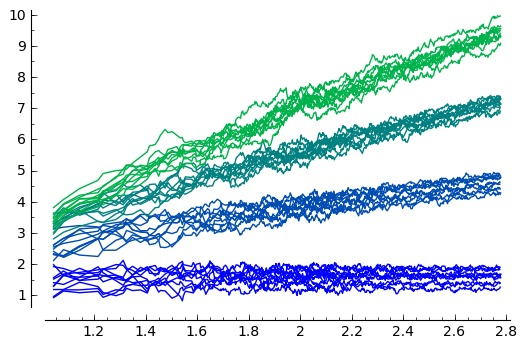
\includegraphics[width=0.7\textwidth]{bsd.jpg}
 \end{center}
 \caption{Oh look, something happens here !}
 \label{fig:bsd}
\end{figure}

\section{Conclusions} \label{sec:conclusions}

Further help on \LaTeX\ can be found easily on the internet. The \LaTeX\
wikibook\footnote{\tt http://en.wikibooks.org/wiki/LaTeX} contains a lot.
For instance you would find there how to type theorems and proofs nicely.
Or how to include source code written in some programming language like
python. There are long lists available with all sorts of common
mathematical symbols like $\xi$, $\nabla$, $\infty$, $\log$, $\iff$, etc.

\newpage

\appendix

\section{Raw data} \label{app:rawdata}

Material that needs to be included but would distract from the main
line of presentation can be put in appendices.
Examples of such material are raw
data, computing codes and details of calculations.

But note tha the maximal number of pages includes the appendix and the references.

\section{Calculations for section \ref{sec:my1}} \label{app:calculations}

In this appendix we could verify equation \eqref{eq:myeq1} or present the code that was used. 
\begin{lstlisting}[language=Python]
def gcd(a,b):
    """
    Return the greatest common divisor
    of a and b 
    """
    while b > 0:
        (a, b) = (b, a % b)
    return a
\end{lstlisting}
 
\newpage

\begin{thebibliography}{99} % alternatively use BibTeX

\bibitem{alling-greenleaf}
N.~L. Alling and N.~Greenleaf,
{\it Foundations of the Theory of Klein Surfaces\/},
Lecture Notes in Mathematics Vol.~219
(Springer, Berlin, 1971).

\bibitem{barrett-dawe}
J.~W. Barrett and R.~A. Dawe Martins,
``Non-commutative geometry and the standard model vacuum'',
{\it J. Math.\ Phys.\ \bf 47}, 052305 (2006).
(arXiv:hep-th/0601192)

\bibitem{bott-tu}
R.~Bott and L.~W. Tu,
{\it Differential Forms in Algebraic Topology\/}
(Springer, New York, 1982).

\bibitem{dewitt-can}
B.~S. DeWitt,
``Quantum theory of gravity. I. The canonical theory'',
{\it Phys.\ Rev.\ \bf 160}, 1113--1148
(1967).

\bibitem{giulini-thesis}
D.~Giulini,
``3-manifolds in canonical quantum gravity'',
PhD Thesis,
University of Cambridge (1990).

\bibitem{hatcher}
A.~Hatcher,
{\it Algebraic Topology\/}
(Cambridge University Press, Cambridge, 2002),
Proposition 1.40 and Exercise 1.3.24.

\bibitem{haw-ell}
S.~W. Hawking and G.~F.~R. Ellis,
{\it The Large Scale Structure of Space-Time\/}
(Cambridge University Press, Cambridge, 1973).

\bibitem{krasnov-louko}
K.~Krasnov and J.~Louko,
``$\mathrm{SO}_0(1,d+1)$ Racah coefficients: Type I representations'',
{\it J. Math.\ Phys.\ \bf 47}, 033513 (2006).
(arXiv:math-ph/0502017)

\bibitem{langlois-thesis}
P.~Langlois,
``Imprints of spacetime topology in the Hawking-Unruh effect'',
PhD Thesis, University of Nottingham (2005).
(arXiv: gr-qc/0510127)

\bibitem{poisson-livrev}
E.~Poisson,
``The motion of point particles in curved spacetime'',
{\it Living Rev.\ Relativity \bf 7} 6 (2004),
URL : \texttt{http://www.livingreviews.org/lrr-2004-6} (cited on 31 August 2006).
(arXiv: gr-qc/0306052)

\bibitem{poisson-gr17}
E.~Poisson,
``The gravitational self-force'',
in
{\it Proceedings of the
17th International Conference on General
Relativity and Gravitation\/} (Dublin, Ireland, July 18--23, 2004),
edited by
P.~Florides, B.~Nolan and A.~Ottewill
(World Scientific, Singapore, 2005) 119--141.
(arXiv:gr-qc/0410127)

\bibitem{wheeler-geon}
J.~A. Wheeler,
``Geons'',
{\it Phys.\ Rev.\ \bf 97}, 511--536
(1955).

\bibitem{wolf}
J.~A. Wolf,
{\it Spaces of Constant Curvature\/},
5th edition
(Publish or Perish, Wilmington, 1984).


\bibitem{ligo-site}
Website \texttt{http://www.ligo.caltech.edu/},
visited 14 August 2007.

\end{thebibliography}

\end{document}
